\documentclass[a4paper]{report}
\usepackage[T1]{fontenc}
\usepackage{lmodern}
\usepackage{amssymb,amsmath}
\usepackage{ifxetex,ifluatex}
\usepackage{fixltx2e} % provides \textsubscript
% use microtype if available
\IfFileExists{microtype.sty}{\usepackage{microtype}}{}
\ifnum 0\ifxetex 1\fi\ifluatex 1\fi=0 % if pdftex
  \usepackage[utf8]{inputenc}
\else % if luatex or xelatex
  \usepackage{fontspec}
  \ifxetex
    \usepackage{xltxtra,xunicode}
  \fi
  \defaultfontfeatures{Mapping=tex-text,Scale=MatchLowercase}
  \newcommand{\euro}{€}
\fi
\ifxetex
  \usepackage[setpagesize=false, % page size defined by xetex
              unicode=false, % unicode breaks when used with xetex
              xetex]{hyperref}
\else
  \usepackage[unicode=true]{hyperref}
\fi
\hypersetup{breaklinks=true,
            bookmarks=true,
            pdfauthor={},
            pdftitle={},
            colorlinks=true,
            urlcolor=blue,
            linkcolor=maroon,
            pdfborder={0 0 0}}
\setlength{\parindent}{0pt}
\setlength{\parskip}{6pt plus 2pt minus 1pt}
\setlength{\emergencystretch}{3em}  % prevent overfull lines

\setcounter{secnumdepth}{1}
\setcounter{tocdepth}{1}

\title{Hacking Education with Virtual Microworlds}
\author{Pascal Chatterjee}

\begin{document}

\maketitle

\begin{abstract}
Contrary to popular belief, the scientists working in their laboratories are not the members of society who learn the most in their daily lives. The members of society who do \textit{by far} the most learning in their daily lives are children. 

Children tend to walk by the age of 18 months; they can express themselves in the extremely complex system known as natural language by the age of two years; and they have developed a theory of mind after spending a mere four years in the world. And they manage all of this before entering formal education.

The progress of even the hardest working university student pales in comparison. This is not just due to the difference in age between adults and children. It also has to do with the environment in which we learn.

Microworlds are environments in which adult minds can \textbf{construct} knowledge in a similar way to children. This paper explains the ideas behind microworlds, describes two implementations of them, and discusses whether they worked and if they will ever be a feature of mainstream curricula. 

The microworld created for this paper, \textit{Narrative Roulette}, is both an engaging and effective learning environment for teenage students. But it won't be until teachers have the technical skills to deeply understand virtual microworlds, and authorities believe in constructionist learning, that microworlds will be adopted by the mainstream.
\end{abstract}

\tableofcontents

\chapter{Ideas}

\section{What is a microworld?}

Imagine you're really hungry. It's late in the day and you need to
decide what you're doing for dinner. This is a problem faced by most of
us, repeated day after day.

What does the solution space look like? The usual way to figure this out
is by examining a single solution and then seeing how its properties
might vary.

A single solution to the whats-for-dinner problem is a single meal. So
the solution space encompasses everything that can be considered a
single meal: everything from a steak to a snack bar. And of course
there's the null solution: not to eat anything at all.

\subsection{Open-ended goals: Creativity within constraints. Coming up
with a \textbf{creative idea}.}

We explore this solution space every time we plan a meal. We work under
certain constraints, such as availability, our personal preferences,
diet plans and even the cultural acceptance of the meal in question. The
set of things we are likely to eat is far smaller than the set of all
things that we \emph{could} eat.

That said, we can also be creative with our solutions. Though our goals
must conform to a certain shape (say roughly 1000 calories of
nutrition), they are also \textbf{open-ended}. There are an infinite
number of ways to get 1000 calories of nutrition, even taking into
account all of the constraints we just mentioned.

Of course, we rarely think about all of these possibilites. We tend to
stick to what we know, reducing an infinite vastness to the comfortably
familiar.

I cook pasta a \emph{lot}, and I doubt I'm the only one.

If I decide to combine pasta with bacon and pesto, I have come up with a
potential solution to the whats-for-dinner problem. I call this a
creative idea in the solution space.

To realise my creative idea, I have to cook.

\subsection{Implementation}

How will I fry the bacon? Shall I make pesto myself or buy it in a jar?
What kind of pasta shall I use, and how should I prepare it?

When I make these decisions, I am trying to realise my abstract idea
with a concrete implementation. I am turning a creative idea in my head
into something I can put on my plate.

\subsection{Evaluation}

Once my reified idea is on my plate, the evaluation phase begins. If my
solution contains roughly 1000 calories, we can call it a meal. But is
it a satisfactory one?

Like the solution space, the evaluation space is infinite. I may have
achieved my nutritional goals, but failed my goals of taste. Or maybe my
meal was both nutritious and tasty, but it just wasn't \emph{novel}
enough.

We might call judging a meal hopelessly subjective. One person's
delicacy is another person's travesty. Yet certain dishes achieve global
popularity. The owners of the most famous restaurants probably believe
that the popularity of a certain dish can be reliably predicted.

\subsection{Feedback and iteration}

An evaluation of the implementation of a creative idea is only useful if
it guides future actions.

Imagine I feel that my home-made pesto failed utterly. This is only a
productive thought if the next time I plan a meal, I change the way I
acquire pesto. Either I change how I make it, or I buy it ready-made
from the supermarket. The success of my updated method will only be seen
when I taste my new, modified meal.

In this way I can learn about what succeeds and what fails.

\subsection{Learning as a process}

\textbf{Learning is what happens when someone executes an
idea-implementation-evaluation loop, and uses outcomes to guide future
iterations.}

\textbf{A microworld is an environment that enables a person to iterate
an idea-implementation-evaluation loop within a certain domain.}

A supermarket, kitchen and dinner table is a microworld for meals.

\section{What kinds of microworld exist today?}

By the age of 21, the average young person will have spent as much time
playing video games as they will have spent in a classroom \{ted\}.
Their presence in the classroom is required by law. Their presence in
front of the screen is entirely voluntary.

\subsection{What is a game?}

So what exactly is a game, and what lets them demand such attention from
children and young adults?

According to Jane McGonigal, a game designer and writer, the four
defining traits of a game are the following:

\begin{enumerate}[1.]
\item
  The \textbf{goal} is the specific outcome that players will work to
  achieve. It focuses their attention and continually orients their
  participation throughout the game. The goal provides players with a
  sense of purpose.
\item
  The \textbf{rules} place limitations on how players can achieve the
  goal. By removing or limiting the obvious ways of getting to the goal,
  the rules push players to explore previously uncharted possibility
  spaces. They unleash creativity and foster strategic thinking.
\item
  The \textbf{feedback system} tells players how close they are to
  achieving the goal. It can take the form of points, levels, a score,
  or a progress bar. Or, in its most basic form, the feedback system can
  be as simple as the players' knowledge of an objective outcome: ``The
  game is over when . . .'' Real-time feedback serves as a promise to
  the players that the goal is definitely achievable, and it provides
  motivation to keep playing.
\item
  Finally, \textbf{voluntary participation} requires that everyone who
  is playing the game knowingly and willingly accepts the goal, the
  rules, and the feedback. Knowingness establishes common ground for
  multiple people to play together. And the freedom to enter or leave a
  game at will ensures that intentionally stressful and challenging work
  is experienced as \emph{safe} and \emph{pleasurable} activity.
  \emph{Taken from ``Reality is Broken''\{rebroken\}, by Jane McGonigal,
  emphasis hers.}
\end{enumerate}

To summarise, a game comprises of the \textbf{voluntary} attempt to
achieve a certain \textbf{goal}, according to a set of \textbf{rules},
with \textbf{feedback} on how close you are to that goal.

\subsection{Are games microworlds? Or are microworlds games?}

Let's compare this with our definition of a microworld, from the
previous section. A microworld is an environment that supports a loop
comprising of:

\begin{enumerate}[1.]
\item
  An \textbf{idea} that a student comes up with \emph{themselves}.
\item
  An \textbf{implementation} of that idea, according to the \emph{rules}
  of the microworld.
\item
  An \textbf{evaluation} of the implementation, that gives the student
  \emph{feedback} about the quality of their implementation and idea.
\item
  The evaluation generates further ideas, and the loop continues.
\end{enumerate}

As we can see, there seems to be an isomorphism between microworlds and
games. An \textbf{idea} in a microworld corresponds to a \textbf{goal}
that a student chooses \textbf{voluntarily}. The \textbf{implementation}
of that idea must conform to certain \textbf{rules}, set by the
\emph{structure} of the microworld. And the purpose of
\textbf{evaluating} a student's implementation is to give them
\textbf{feedback} about it, so they can improve their future ideas.

But the two are not exactly equivalent, as a microworld's \textbf{idea}
conflates the \textbf{voluntary} and \textbf{goal} traits of a game.
Every microworld is a game (each microworld contains all four traits of
a game), but not all games are microworlds.

\begin{quote}
Only those games that allow the voluntary choice of goals can be
considered microworlds.
\end{quote}

\subsection{Flappy Bird vs Minecraft}

Wikipedia says this about the gaming phenomenon known as Flappy Bird
\{3\}:

\begin{quote}
Flappy Bird is a side-scrolling mobile game featuring 2D retro style
graphics. The objective is to direct a flying bird, which moves
continuously to the right, between each oncoming set of pipes without
colliding with them, which otherwise ends the game. The bird briefly
flaps upward each time the player taps the screen. If the screen is not
tapped, the bird falls due to gravity. The player is scored on the
number of pipe sets the bird successfully passes through, with medals
awarded for the score.
\end{quote}

Though players play Flappy Bird \textbf{voluntarily}, they have no say
in their \textbf{goal}. They just have to keep flapping, or they die and
the game is over. The simplicity of Flappy Bird's \textbf{rules} (just
flap) and the sophistication of its \textbf{feedback system} (if I'd
flapped \emph{slightly} earlier, I'd be alive!) are what make the game
addictive \{forbes\}.

This means that Flappy Bird qualifies as a game, but not as a
microworld.

Minecraft, on the other hand, is defined by Wikipedia as:

\begin{quote}
Minecraft allow{[}s{]} players to build constructions out of textured
cubes in a 3D procedurally generated world. Other activities in the game
include exploration, gathering resources, crafting, and combat. Gameplay
in its commercial release has two principal modes: survival, which
requires players to acquire resources and maintain their health and
hunger; and creative, where players have an unlimited supply of
resources, the ability to fly, and no health or hunger.
\end{quote}

The goal of Minecraft's \textbf{survival} mode is, unsurprisingly, to
survive. This goal is non-negotiable. However, Minecraft also has
another mode, in which players have neither health nor hunger. This
means that there is only one reason for playing this mode of the game:
the joy of building things from virtual, textured cubes.

In this particular case, of a specific mode of a specific game, we have
an environment in which players can \emph{choose their goals with total
freedom}. This makes Minecraft's \textbf{creative} mode a model example
of something that is both a game and a microworld.

\subsection{What other activities can be microworlds?}

We've established that microworlds are a subset of games - those
activities that contain all four of McGonigal's traits listed above. Of
course, the set of all games is wider than just video games. Let's look
at some other activities that could be described as microworlds.

\subsubsection{Jamming}

Consider a few people gathering in a room, each with their own musical
instrument, jamming together. There is a \textbf{goal}: to make music
that sounds good. There are \textbf{rules} (or \emph{constraints}): of
timing (4 beat bars), chord sequences that sound good together, the
traditions of the genre, the expectations of the potential audience,
etc. \textbf{Feedback} is instant: the musicians can tell if something
sounds good, \emph{while they're playing it}. And of course, jamming is
\textbf{voluntary} in the vast majority of cases.

This means that jamming is actually a game, even though we wouldn't
usually describe it that way. Is jamming also a microworld?

For a game to also be a microworld, it has to allow voluntary choice of
\textbf{goals}. Though the overarching goal of jamming is to make good
music, the group can work towards that with subgoals.

Perhaps the group decide the first step is to come up with a catchy
chorus. The guitarist might have some ideas for chords she wants to try;
the singer has some idea of what words he wants to sing; the drummer has
some ideas about a beat, and so on.

These \textbf{ideas} are \textbf{implemented} immediately, and
\textbf{evaluated} soon after, by the musicians who judge whether what
they're doing is working. If it isn't, they update their \textbf{ideas}:
the drummer tries a different beat, or the guitarist switches chords,
and they iterate. Otherwise, they move on to another part of the song.

In this light, jamming can be described as a microworld, as it shares
its basic structure with something like Minecraft, even though, on the
surface, the two activities look very different.

\subsubsection{Creative writing}

Writing fiction is a microworld too. A lone writer has an \textbf{idea}
in her head for a story. It probably isn't the whole story, word for
word, fully-formed in her head. It's probably a rough idea, like:
``dinosaurs on the loose in zoo, people try to escape'' or ``criminal
couple rob banks and are then shot by the police''.

The smaller ideas that make up this grand vision might be: ``the people
escaping the dinosaurs are archaeologists'', or ``wouldn't it be cool to
have a scene where a rampaging tyrannosaurus rex destroys a skeleton of
its own species?''.

The \textbf{implementation} of these ideas takes the macro form of
scenes, characters and events; and the micro form of the words used to
describe them. \textbf{Evaluation} occurs when the writer reads back
what she's written, a process that the author David Foster Wallace once
called ``feed{[}ing{]} the wastebasket''\{flesh\}.

Again, this makes writing a game, and the free choice of goals, or
ideas, makes it a microworld too.

\subsubsection{Programming}

The microworld of programming is the one I have most experience with. An
\textbf{idea} in this world could be something like: ``I want to build a
system where users can vote for things''. Smaller ideas could be: ``the
system should work on mobile phones'' and ``the page should update by
itself''.

An \textbf{implementation} could use a HTML5 front-end, a Python
back-end, and HTTP and WebSockets to communicate between them.

The \textbf{evaluation} would be testing the system, first in unit and
end-to-end automated tests, and finally by real users in a production
environment.

Iterating this loop at speed is known as \textbf{extreme
programming}\{wiki:extreme\} (although as with all programming jargon,
its exact meaning is hard to pin down).

\textless{}\textless{} THE REPL IS A MICROWORLD
\textgreater{}\textgreater{}

\subsection{Degrees of Microworld}

So we have a bunch of environments that we think are microworlds:
sandbox video games (like Minecraft), jamming, creative writing and
programming. They all seem to be games (or at least have the potential
to be), and as ideas can be chosen freely, we argue that they are
microworlds too.

But how ``free'' are they, and if we gradually restrict this freedom,
will we eventually end up with things that are no longer microworlds?

Let's take our programming example. Imagine the project is a commercial
one, paid for by a client with certain requirements. These requirements
include: * The front-end must look exactly like the given mockups. * The
front-end must be an iOS app. * The back-end must be written in Java,
and use servlets. * The entire project must be production ready within a
week.

Do we still have a microworld? The person or team working on the project
is severely restricted in what \textbf{ideas} they can have. They have
to conform to the mocked-up design, write it in the specified front and
back-end languages, and can only do things that will fit in the given
time-frame.

As a result, the solution space is extremely narrow; there's probably
only a few ways to do anything, and maybe only one that could work given
all the constraints. So the team only really \textbf{implement}, and the
client is the one who will \textbf{evaluate}.

Just implementing does not a microworld make. It doesn't even qualify as
a game, as participation is not \textbf{voluntary}, and the
\textbf{feedback system} is probably far from real-time.

\begin{quote}
The more freedom allowed in an activity, the more of a microworld it is.
\end{quote}

Ideally, the only constraints are those imposed by the structure of the
microworld: in programming we are limited by our technology; in writing
or music we are limited by our own abilities and the culture in which we
live.

But an activity can still be a microworld, even if we have a deadline
and have some constraints over those imposed by the environment. Writing
a story can still be a microworld even if it has to be done by the end
of the month, and must include dinosaurs and a happy ending.

Because the solution space is still wide-open; \textbf{ideas} can still
be had. But once scenes, characters and actions start being heavily
constrained, the potential for \textbf{ideas} will reduce, and the
microworld will become just another job.

NEXT: So we know what microworlds are, and which ones exist today. What
evidence do we have that they enable learning?

\begin{center}\rule{3in}{0.4pt}\end{center}

\{ted\} Jane McGonigal
\href{http://www.ted.com/conversations/44/we\_spend\_3\_billion\_hours\_a\_wee.html}{http://www.ted.com/conversations/44/we\_spend\_3\_billion\_hours\_a\_wee.html}
\{rebroken\} Jane McGonigal ``Reality is Broken'' \{wiki:flappy\}
Wikipedia Flappy Bird \{forbes\}
http://www.forbes.com/sites/ewanspence/2014/02/18/the-vital-and-depressing-lessons-flappy-bird-can-teach-indie-developers/
\{flesh\} Both Flesh And Not, David Foster Wallace \{wiki:extreme\}
Wikipedia Extreme Programming

\section{Microworlds enable learning}

\subsection{John Dewey}

99 years ago, John Dewey, a philosopher of education, wrote:

\begin{quote}
``{[}\ldots{}{]} the school in turn will be a laboratory in which the
student of education sees theories and ideas demonstrated, tested,
criticized, enforced, and the evolution of new truths.''\cite[p55]{dewey}
\end{quote}

Dewey conceived of a school consisting of laboratories and studios,
where students would be able to construct things and experiment with
their own hands, instead of constantly being told what to do
and how to do it.

He wanted to see \textbf{ideas} demonstrated (or \textbf{implemented});
tested and criticized (or \textbf{evaluated}); for the evolution of new
truths (or the updating of ideas through iteration).

\subsection{Jean Piaget}

According to Edith Ackermann's analysis of the work of Jean Piaget:

\begin{quote}
``To Piaget, knowledge is not information to be delivered at one end, and
encoded, memorized, retrieved, and applied at the other end. Instead,
knowledge is experience that is acquired through interaction with the
world, people and things.''\cite{ackermann}
\end{quote}

This is because, to Piaget (according to Ackermann):

\begin{quote}
``Kids don't just take in what's being said. Instead, they interpret what
they hear in the light of their own knowledge and experience.''\cite{ackermann}
\end{quote}

Imagine an adult and child standing near a fire. According to
Ackermann's analysis of Piaget, Piaget would say that the child will not
refrain from touching the flame just because the adult tells the child
it will burn their hand (they ``don't just take in what's being said'').

Once the adult has gone, the child will reach for the flame regardless.
They will only abort their attempt to touch the fire once its heat on
their hand becomes uncomfortable (adding ``their own knowledge and experience'' to what they've been told).

Here is our first hint at \emph{why} microworlds could be useful for
learning. It's because microworlds are environments in which rich
experiences can be had (experiences such as those described by Dewey).
Microworlds are also safe places to have those experiences - hurting
yourself in a game is far less painful than doing so in real life.

\subsection{Seymour Papert}

\begin{quote}
``Constructionism means "Giving children good things to do so that they
can learn by doing much better than they could before." {[}\ldots{}{]}
Instructionism is the theory that says, "To get better education, we
must improve instruction."''\cite{convsinst}
\end{quote}

\begin{quote}
``Constructionism {[}\ldots{}{]} shares constructivism's connotation of
learning as "building knowledge structures" irrespective of the
circumstances of the learning. It then adds the idea that this happens
especially felicitously in a context where the learner is consciously
engaged in constructing a public entity, whether it's a sand castle on
the beach or a theory of the universe.''\cite{sitconst}
\end{quote}

Piaget thought that knowledge is \textbf{constructed} by the learner: we
build \textbf{knowledge structures} in our minds, from concrete
experiences - interactions with the world, people and things. This is called ``constructivism''.

Papert added to this theory, to come up with what he calls
``constructionism'' - the idea that knowledge structures are best
constructed when the learner is building a \emph{public} entity.

I believe the inclusion of the word ``public'' is important. I think it
has to do with the \textbf{evaluation} stage of our microworld loop.

If an entity is public, it will be evaluated in public, by more people
than its creator. This allows for richer feedback than if the creator
was the sole person in charge of evaluating their work.

In practice, this means that products of microworlds (whether they are
songs, stories or programs) should be exhibited to maximise the value of the feedback received by the creator of the work.

\begin{quote}
``Now one can make two kinds of scientific claim for constructionism. The
weak claim is that it suits some people better than other modes of
learning currently being used. The strong claim is that it is better for
everyone than the prevalent ``instructionist'' modes practiced in
schools. A variant of the strong claim is that this is the only
framework that has been proposed that allows the full range of
intellectual styles and preferences to each find a point of equilibrium.''\cite{sitconst}
\end{quote}

Microworlds allow students to construct knowledge \emph{in their own
way}. They offer building blocks that each student can use to construct knowledge in their own
personal style. 

The ``instructionist'' framework of traditional educational does not allow this. When you are being told how to do things, you need to follow the rules set by the instructor, not those that you come up with yourself.

\subsection{What do microworlds reward?}

Let's look at what microworlds reward in their users. To understand
this, we should look at the Papertian public entities that would be
constructed within these microworlds.

Consider Minecraft. Fans of the TV and book series \emph{Game of
Thrones} have built a version of Westeros, the series' fantasy realm,
from 1.2 billion bricks. Compared to the size of the characters, this
Minecraft construction is the size of Los Angeles\cite{westeroscraft}.

Creating something the size of Los Angeles, even if it only exists in
cyberspace, requires considerable skill. Builders need to be able to
place single blocks to form superstructures, and compose those
superstructures to form hyperstructures, and so on\cite{reddit:minecraft}.

When shared on servers, Minecraft artifacts are public entities. How are
these evaluated by other members of the public? Like other works of art.
It appears that complexity for its own sake is not admired; non-trivial
complexity must be twinned with aesthetic beauty for an artifact to be
admired\cite{mash}.

The same can be said of the creative writing microworld. Ralph Ellison, the American novelist, has said: ``Good
fiction is made of what is real, and reality is difficult to come by,''
which can be interpreted as saying that writing fiction rewards non-trivial ``truth'' value, instead of mere complexity.

Playing Flappy Bird, on the other hand, rewards (non-trivial) hand-eye coordination. A public entity in the
Flappy Bird world is a player's high score. Using this as a
feedback mechanism does increase your hand-eye coordination, in a very narrow domain,
but does not improve much else. 

\subsection{How do these rewards lead to learning?}

During iterations of the microworld loop in the microworlds mentioned, you do the following:

\begin{itemize}

\item You build complex superstructures in Minecraft\cite{local:minecraft}.
\item You think creatively and express yourself in natural language when writing fiction\cite{neural}.
\item You time your flaps in Flappy Bird.

\end{itemize}

There is a learning algorithm in the field of Artificial Intelligence called \textbf{Reinforcement Learning}. It can be described as follows:

\begin{quote}
``[An agent] must discover which actions yield the most reward by trying them. In the most interesting and challenging cases, actions may affect not only the immediate reward but also the next situation and, through that, all subsequent rewards.''\cite{reinforcement}
\end{quote}

By carrying out actions in its environment, evaluating rewards and iterating, an agent \emph{learns}. If we accept that this applies to human agents as well as artificial ones, we must conclude that iterating the microworld loop within microworlds enables learning too.

Therefore, the rewards in the environments mentioned lead to learning in the following ways:

\begin{itemize}

\item Building in Minecraft makes you better at creating complex superstructures.
\item Writing fiction makes you better at thinking creatively and expressing yourself.
\item You get better at timing your flaps in Flappy Bird.

\end{itemize}

The first two environments, Minecraft and creative writing, seem to lead to \emph{deeper} learning than Flappy Bird. This is because they are microworlds as well as being games. That said, the mechanism by which learning takes place is the same - reinforcement learning.

\section{Microworlds are engaging}

\subsection{What is the key to motivation?}

According to Dan Pink, it's autonomy. Roman Krznaric agrees, and uses
the following statistic to prove his point: 47\% of self-employed people
say they are ``very satisfied'' with their jobs, compared to only 17
percent of those in regular employment\{krznaric\}.

Here is the table from which he got his data\{joywork\}:

\% of respondents Full-time Part-time Self-employed Very dissatisfied
5.8 3.2 1.6 Dissatisfied 11.2 10.5 4.7 Neutral 18.7 18.9 12.5 Satisfied
46.9 48.4 34.4 Very satisfied 17.3 18.9 46.9

There are more than twice as many dissatisfied people working full time
compared to those who are self-employed.

Why would this be?

The report has this to say:

\begin{quote}
This could be attributed to the control that the self-employed have over
their work: whilst many work very long hours, their ability to determine
when, where and how they work may contribute to their high levels of
satisfaction.
\end{quote}

If you have the ``ability to determing when, where and how'' you work,
that means you have autonomy over your work.

\subsection{Do microworlds provide autonomy?}

The first stage of our microworld-defining loop is coming up with an
\textbf{idea} that obeys the constraints of the \emph{structure} of that
microworld.

Imagine you are a self-employed, freelance web designer. You have been
tasked with coming up with a new landing page for a coffee shop brand.

You have autonomy over when you work, where you work, and how you work.
You can work only between 22.00 and 04.00. You can work from home. You
can use or skeumorphic design, or flat design.

Let's say you try skeumorphic design, but after you \textbf{implement}
some skeumorphic elements, and \textbf{evaluate} them, something seems
off. You update your \textbf{ideas} and try flat design instead. Much
better.

You exercised your autonomy in \emph{how} you work.

But however much you iterate, you still need to deliver something that
looks like a web page. You can't deliver a design for a printed book. Or
a design for a 15-minute movie.

Those are the constraints of the \emph{structure} of your web design
microworld.

\subsection{What would a microworld look like without autonomy?}

Let's imagine our web design microworld without autonomy.

Your task is still the same: creating a landing page for a coffee shop
brand.

But this time, you must work between 09.00 and 17.00 on weekdays. You
must work from the office, from your cubicle. You're free to use
skeumorphic design or flat design\ldots{} but your boss \emph{really}
likes skeumorphic design.

After \textbf{implementing} your initial skeumorphic design
\textbf{idea}, you \textbf{evaluate} it, and as before, you find it
lacking.

Unfortunately, you can't change it. Because your boss likes it, and
their opinion overrules yours.

The structural constraints of the microworld still apply. But now some
arbitrary constraints \emph{also} apply: over where, when and how you
work.

These additional, arbitrary constraints suck the fun right out of the
microworld. They make the microworld less engaging. They make it feel
like work, not a game.

\subsection{What does engagement lead to?}

When a microworld allows for autonomy, it is a highly motivating place
to experiment in.

In Minecraft, this motivation leads to people building their first basic
block structure. For a band jamming together, or a novice writer, it
might lead to the first work they're comfortable sharing with friends.
For the budding programmer, it usually leads to their first non-trivial,
mostly-working program.

And that leads to a sense of accomplishment. But that's not where it
ends.

After an initial success, the temptation is there to tweak the original,
ever so slightly. The first block structure leads to a house; one song,
story or program leads to another, similar in structure but differing in
detail.

Eventually, we end up with a blockrealm the size of Los Angeles; a band
and author with a string of hits; a programmer in charge of a program
that serves billions around the world.

As we argued in the previous section, each iteration of our loop led to
learning for all involved.

But it took the engagement enabled by autonomy to start the loop
spinning in the first place.

\ctable[pos = H, center, botcap]{ll}
{% notes
}
{% rows
\FL
\parbox[t]{0.07\columnwidth}{\raggedright
\{krzn \{joyw
} & \parbox[t]{0.26\columnwidth}{\raggedright
aric\} How To Find Fulfilling Work ork\}
\href{http://twfold.theworkfoundation.com/assets/docs/publications/145\_Joy\_of\_Work.pdf}{http://twfold.theworkfoundation.com/assets/docs/publications/145\_Joy\_of\_Work.pdf}
}
\LL
}

\section{Virtual microworlds}

Unlike our jamming and creative writing microworlds, Minecraft is a
\emph{virtual} microworld. This means that software is an integral part
of the microworld, in a way that is not necessarily true for mostly
physical microworlds.

How does software change things? It eliminates routine tasks, by
delegating those to the machine. Let's see how that works in practice:

The physical microworld equivalent of Minecraft is a pile of Lego bricks
on the floor. Unlike Minecraft, everything is, understandably, manual.
The only way to search for certain kinds of bricks is by conducting a
linear search, or, if you're very organised, sorting the bricks first.

There is a limit to the number of bricks the average person can handle.
This limits the complexity of our Lego creations. There are also
constraints of time and space.

Playing with Lego can occupy the entire floor. This means that only
those people with access to the floor can play. Even at the most social
Lego sessions, it's unlikely more than a handful of people will be able
to participate simultaneously.

And before long, the Lego will have to be tidied away. As bricks are
physical, this usually entails breaking up any structures and putting
single bricks back in the box.

Minecraft is different. As the bricks are virtual, they can be sorted
and organised by the machine. They can be practically infinite in
number, and the increasing complexity in structures can be handled by
the user interface treating a grouping of blocks as one.

The environment is virtual too, so bricks don't have to be tidied away
when you're done; their patterns are stored in bits until you're ready
to return. This makes it easier to work on larger-scale projects, as it
eliminates the need to ever start over from scratch.

It also makes it easier for users to collaborate. Builders no longer
have to be friends, or even geographically close to each other, to work
together in the same environment. They just need to be logged in to the
same server. This encourages large-scale collaborative projects.

But software also creates a barrier to entry. To participate in a
virtual microworld, you need specialised equipment - a computer - that
can run it. That said, you need specialised equipment, such as musical
instruments, to participate in physical microworlds too, and it seems
that computers are becoming less and less ``specialised'' as time goes
on.

However, to run a virtual microworld, you also need specialised
\emph{software} to go along with your hardware. For Minecraft, you need
to install the Minecraft software package. For programming microworlds,
you often need to install an interpreter, configure an editor and to set
up a build system.

The easier a microworld is to enter, the greater its potential audience.
The microworlds that are easiest to enter require the least set up of
specialised software on the part of the user.

The web browser is fast becoming less and less specialised. All
computers come with them pre-installed, and most users spend a
significant part of their computer time using them.

Microworlds in the web browser are arguably the most easily accessible
virtual microworlds. Let's take a look at some current examples.

\subsection{CodePen (\href{http://codepen.io/}{http://codepen.io/})}

CodePen is a browser-based virtual microworld for front-end web
development, i.e.~HTML, CSS and JavaScript. The creation view looks like
this:

\begin{figure}[ht!]
\centering
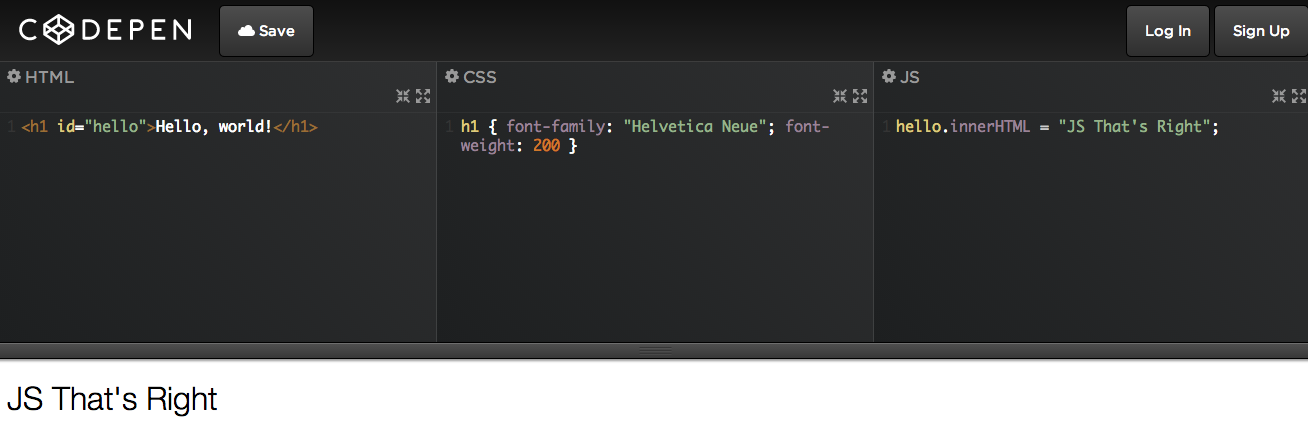
\includegraphics[width=123mm]{img/codepen.png}
\caption{CodePen interface}
\label{overflow}
\end{figure}

There are four panes: one each for HTML, CSS and JavaScript code, and
one that dynamically renders the result.

This microworld leverages the browsers capacity for dynamic rendering:
of parsing and showing the results of code on the fly. A website allows
you to experiment with creating websites.

Created entities in CodePen - ``Pens'' - are public entities and can be
browsed by others, and even tweaked by them. This creates a rich
environment for creativity and experimentation, and as we have argued so
far, a rich source of learning, in this case in the domain of front-end
web technology.

\subsection{Pacemaker (\url{http://pacemaker.net/})}

Pacemaker is an iPad application that is also a virtual, musical microworld. It enables users to remix and edit songs from Spotify, in real-time, by touching the iPad screen.

\begin{figure}[ht!]
\centering
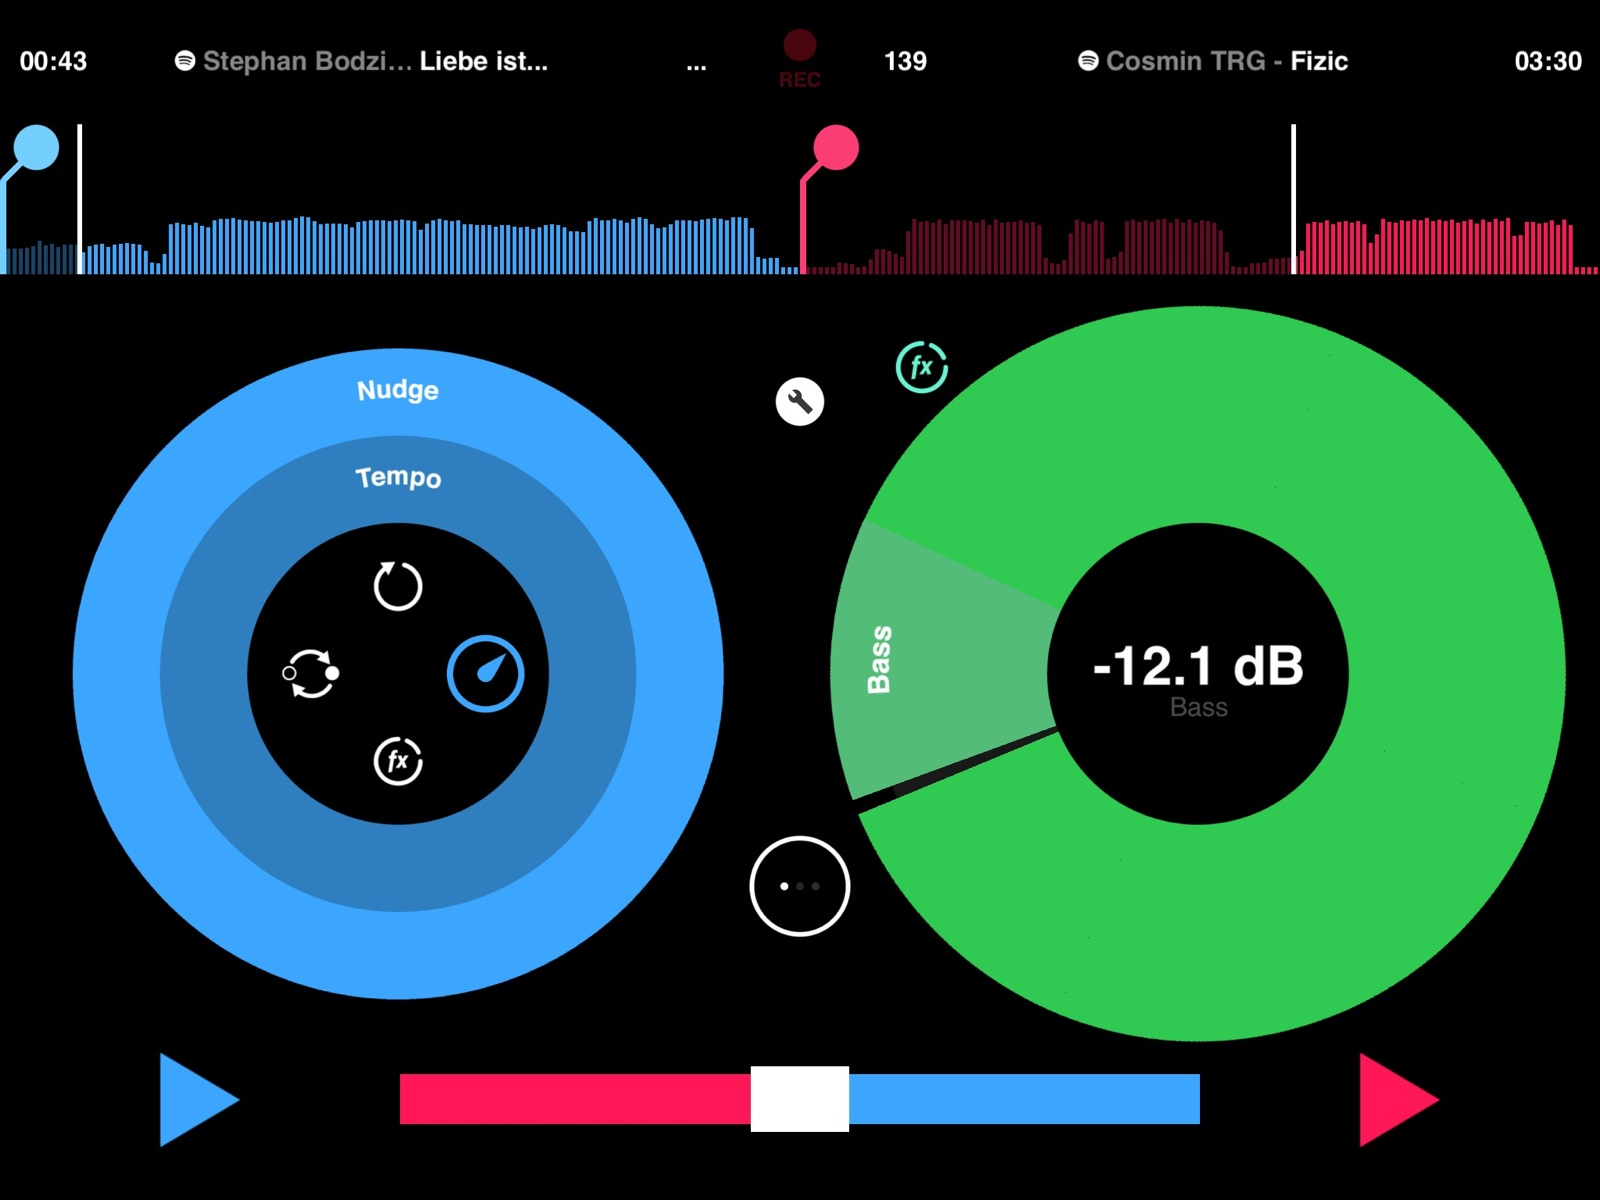
\includegraphics[width=123mm]{img/pacemaker.jpg}
\caption{Pacemaker interface}
\label{overflow}
\end{figure}

Sadly, Pacemaker does not allow sharing of creations, due to copyright issues. But creations can be played back on the iPad that created them so that listeners can evaluate them. 

\subsection{Blogging}

There are many blogging systems on the internet, such as \href{http://wordpress.org/}{Wordpress}, \href{http://tumblr.com}{Tumblr}, \href{http://medium.com}{Medium} and \href{http://ghost.org}{Ghost}. 

Blogging is a virtual microworld where \textbf{ideas} are \textbf{implemented} as text and images, and then (hopefully) \textbf{evaluated} by readers who give feedback by sharing and commenting about blog posts on social media. 

\begin{figure}[ht!]
\centering
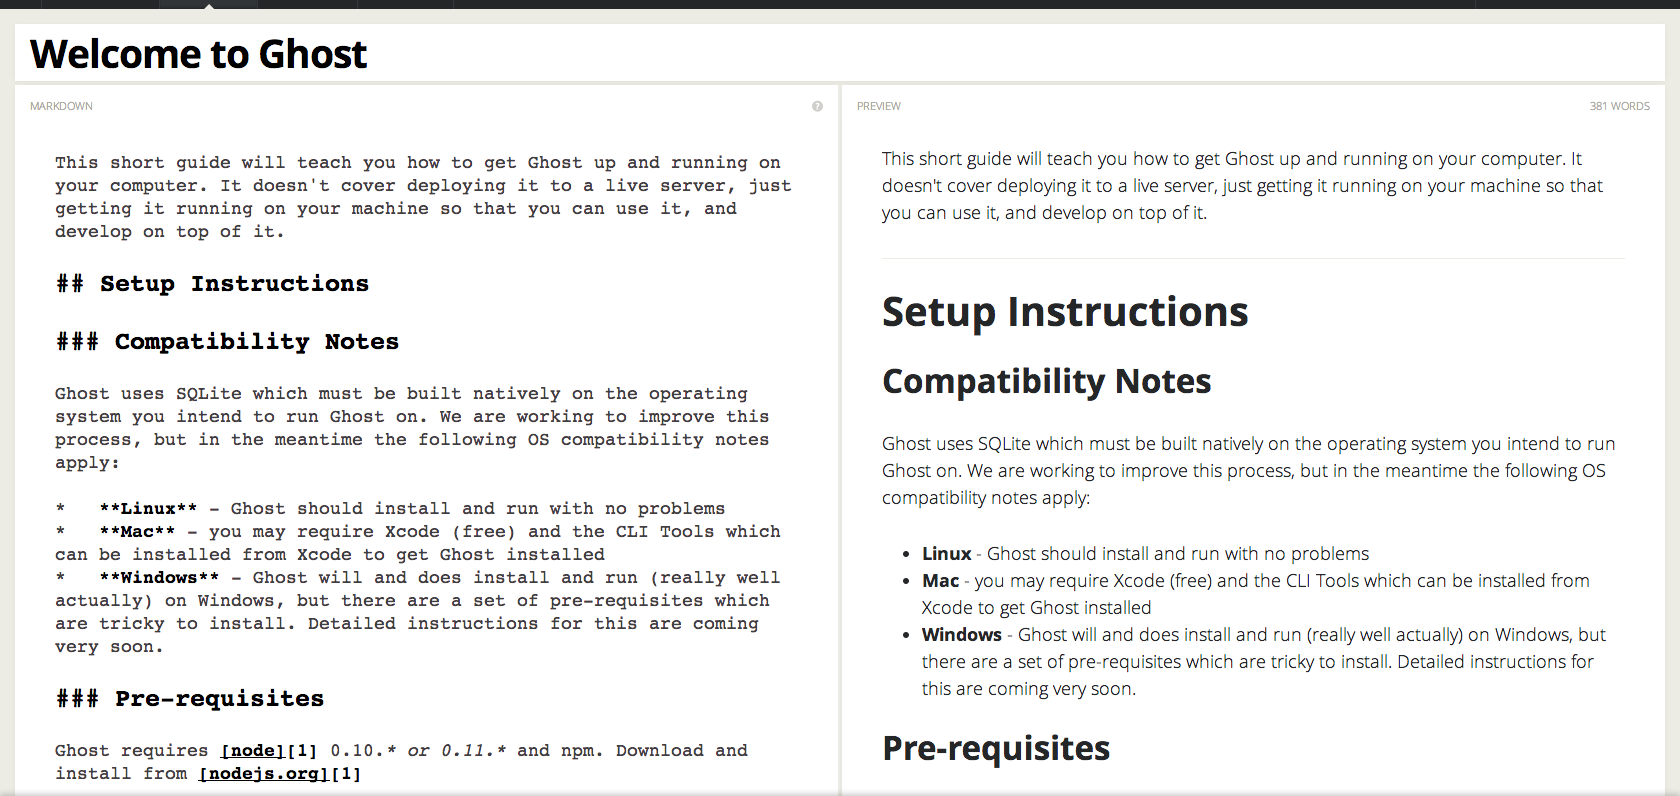
\includegraphics[width=123mm]{img/ghost.png}
\caption{Ghost editing interface}
\label{overflow}
\end{figure}

\subsection{A microworld for microworlds}

According to contructionism, and our sources from the last chapter, the best way for a person to learn about a domain is to construct public entities in that domain. Therefore, the best way for me to learn about microworlds is to build some myself. For the reasons outlined above, I chose to build virtual, browser-based microworlds. 

The next chapter describes these microworlds. 


\chapter{Implementation}

\section{Talking to Machines}

After researching microworlds and developing my theoretical framework, I
felt ready to design my own microworld, which I named \emph{Talking to
Machines}. You can find it online at \url{http://draw.talkingtomachines.org}.

Concretely, this entailed designing an environment in which an
\textbf{idea-implementation-evaluation} loop could be carried out. For the
reasons discussed in the previous section, I decided to host this
environment within the web browser.

This decision brought with it some constraints: the interface would have
to be built from HTML and CSS, and interactivity would have to either be
supplied by client-side JavaScript, or a server-side evaluation
environment. But this decision also enabled the increased accessibility
discussed earlier.

I decided to focus this microworld on programming, as that is an
activity I have a lot of experience with. In a web environment, that
would entail using JavaScript as the programming language, as that is
available on the client-side, and removes the need to execute a
different language on the server and then send back the results.

However, I'm not a great fan of JavaScript when it comes to teaching
beginners to program (see \href{https://www.destroyallsoftware.com/talks/wat}{here}\footnote{https://www.destroyallsoftware.com/talks/wat} for why, from 1:18). Instead, I chose to use
a dialect of Lisp - Clojure (in its JavaScript-hosted form,
ClojureScript) - as Lisp has a history of being a language well-suited
for beginners (MIT has used it in an introductory \href{http://mitpress.mit.edu/sicp/course.html}{programming course}\footnote{http://mitpress.mit.edu/sicp/course.html} for years).

\subsection{From ClojureScript to JavaScript}

At the time of creating \emph{Talking to Machines}, there was no way to
dynamically evaluate ClojureScript in the browser, as the reader and
compiler for ClojureScript forms was in fact a Clojure program that
could only run on the Java Virtual Machine.

The following makes this rather complicated concept a little easier to
understand:

The ClojureScript syntax for printing ``Hello World!'' to the console
looks like this: 

\begin{verbatim}
(.log js/console 'Hello World!')
\end{verbatim}

If ClojureScript could be evaluated in the browser, you'd expect to be
able to do something like this, in \textbf{JavaScript}: 

\begin{verbatim}
ClojureScript.eval("(.log js/console 'Hello World!')") 
\end{verbatim}

and have ``Hello World!'' printed to the console.

Unfortunately, in standard ClojureScript, you can't do that yet.

Instead, a \textbf{Clojure} program, running on the JVM (i.e. not in the browser), has to \textbf{transpile} a ClojureScript file to a
JavaScript file. This means that 

\begin{verbatim}
(.log js/console "Hello World!")
\end{verbatim}

in the Clojurescript file, \texttt{foo.cljs}, is transpiled to

\begin{verbatim}
console.log("Hello World!")
\end{verbatim}

in the output Javascript file, \texttt{foo.js}, by a server-side process run during a compilation phase. 

It is this file, \texttt{foo.js}, that is later evaluated in the web browser.

\subsection{So what does this mess actually mean, practically?}

It means that if a user writes ClojureScript in the browser, we won't be
able to evaluate what they wrote without having a backend Clojure
process transpiling their code to JavaScript for us.

This isn't actually a massive issue, as we still don't evaluate
arbitrary code on the back-end, which would obviously be a Big Deal (we
only transpile it), but it would introduce some network lag
between the \textbf{implementation} and \textbf{evaluation} stages of
our microworld loop.

We know the tighter the microworld loop, the more engaging the experience, so lag was something I wanted to avoid if at all possible.

\subsubsection{Kanaka to the rescue}

Luckily for me, there was a \href{https://github.com/kanaka/clojurescript}{fork of ClojureScript}\footnote{https://github.com/kanaka/clojurescript} that did allow evaluation in the browser, written by Joel Martin
(``Kanaka'' on Github). At the time of writing it is still a fork, and
hasn't been merged with ClojureScript core, probably because it contains
``miscellaneous broken things that have not been tracked down yet''.

But it was definitely good enough to evaluate ClojureScript for a
microworld, and it probably took me less time to modify Martin's code to
provide my wished-for \texttt{ClojureScript.eval} JavaScript function
than it took me to explain why that was necessary.

\subsection{Why did I go to all this trouble?}

This might seem like a very convoluted mess to get into just to avoid
writing pure JavaScript, which, after all, is good enough for sites like
\href{http://codecademy.com}{Codecademy}\footnote{http://codecademy.com}. That's a fair point but I believe that the declarative
purity of ClojureScript forms makes up for the chaos going on behind the
scenes. As you will soon see.

\subsection{A better first impression of programming}

Most very-first-introductions to a programming language, or programming
in general, involve printing the text ``Hello World!'' to the screen.
Later exercises usually include things like printing the numbers ``1 2 3
4 5 6 7 8 9 10'', or adding up all integers less than 100.

Though these feats may have been impressive 30 years ago, today these things fail to blow
most people's socks off.

Producing plaintext is far from unimportant (most webservers do little
else), but in a world where technology means Oculus Rift and 4K Netflix,
it's not really sexy.

Is there something simple we can have beginners do, to explain functions
and variables and loops, that is more interesting than printing text to
the screen?

We could try the activity that captivates children (and artists) all
over the world: drawing things. With colours!

\begin{figure}[ht!]
\centering
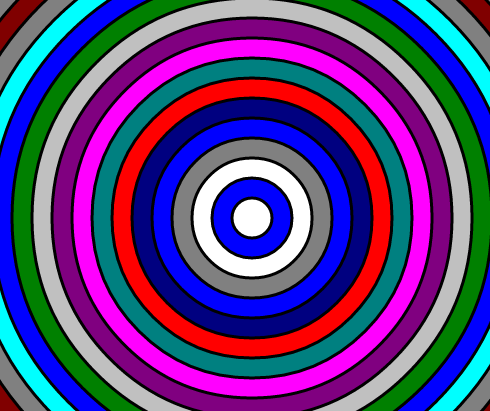
\includegraphics[width=100mm]{img/concentric_circles.png}
\caption{The kind of thing that blows socks off.}
\label{overflow}
\end{figure}

\subsection{Declarative shapes}

The most basic form of computation is a single function call. It is the
simplest action that \emph{does} something (variable assignment does
something too, but indirectly, setting things up for later function
calls).

It makes sense that drawing a shape to a screen should be the result of
just one function call, instead of requiring a novice to construct a
class, call methods on that class, and then draw that class to the
screen after having acquired a graphics context.

The more declarative this function call, the easier it is for a novice
to deduce its meaning from what happens when its evaluated.

Consider: 

\begin{verbatim}
(circle
 (position "50%" "50%")
 (radius 100)
 (fill "red"))
\end{verbatim}

To a non-programmer (and perhaps even a programmer unused to
S-expressions), this line of text looks alien. It conforms to a very
different kind of grammar than what we're used to reading.

This is why, when I ask non-programmers what they think the \texttt{100} in
the line above represents, they often have no idea. The text as a whole
is just too strange for them to parse and guess that the proximity of
\texttt{radius} to \texttt{100}, and the brackets that enclose them, means that the
two tokens have something to do with each other.

If we were in a static environment, the only way to learn about what the
above text does would be to read about the syntax and grammar of Lisp, and the semantics of \emph{Talking to Machines}.
This is often how programming is approached: from a mathematical
perspective. The only way to find out if you had a correct understanding
of syntax, grammar and semantics would be to ask a teacher. The gap between
\textbf{implementation} and \textbf{evaluation} would be so large that
it would kill a lot of your motivation.

Fortunately, \emph{Talking to Machines} is a microworld. This means that
a student can \textbf{evaluate} the above text, right in the browser, to render:

\begin{figure}[ht!]
\centering
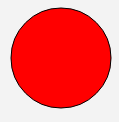
\includegraphics[width=20mm]{img/red_circle.png}
\caption{The meaning of the S-expression}
\label{overflow}
\end{figure}

Then, after processing this visual feedback, the student might have an idea about what the \texttt{(radius 100)} form does, and decide to implement her idea by changing that form to \texttt{(radius 200)}. 

\begin{verbatim}
(circle
 (position "50%" "50%")
 (radius 200)
 (fill "red"))
\end{verbatim}

\begin{figure}[ht!]
\centering
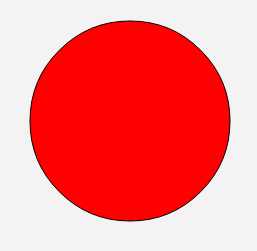
\includegraphics[width=60mm]{img/big_red_circle.png}
\caption{Doubling the radius to 200}
\label{overflow}
\end{figure}

As soon as this modified text is \textbf{evaluated}, a \emph{bigger} circle is drawn on the screen. Immediately, the student realises
that the number that was \texttt{100} but is now \texttt{200} somehow affects the
\emph{size} of the drawn circle.

Through their interactions, the student has \textbf{constructed} this
knowledge for themselves. According to our constructionist learning
theory, this knowledge should be far more effective than being
\emph{told} that the \texttt{(radius 100)} form controls the radius of
the drawn circle.

\subsection{Looping in \emph{Talking to Machines}}

Let's see how \emph{Talking to Machines} supports our microworld loop.

Once a student is somewhat familiar with how the microworld works, they
can come up with the following \textbf{ideas}: 

\begin{itemize}
\item I want to draw a red circle. 
\item Can I make it blue? 
\item Can I make it bigger?
\item Can I move it around? 
\item Can I draw more than one? 
\item Can I draw other shapes? 
\item Can I animate them?
\item etc.
\end{itemize}

Their \textbf{implementations} of these ideas take the form of composed
function calls. These function calls are immediately \textbf{evaluated},
and the student sees visually how their change of code affected the
change in what was drawn to the screen.

\begin{figure}[ht!]
\centering
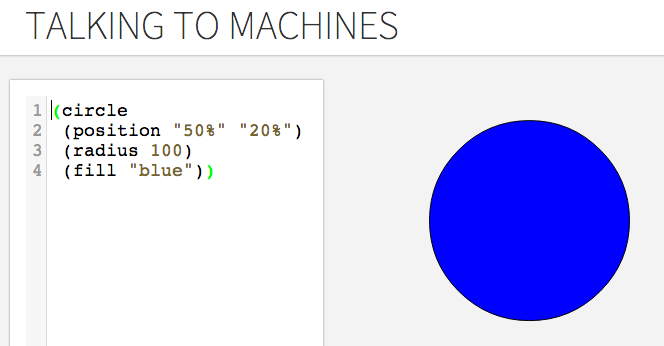
\includegraphics[width=115mm]{img/ttmachines_interface.png}
\caption{The Talking to Machines microworld interface}
\label{overflow}
\end{figure}

For example, the first idea above, of drawing a red circle, looks like
this: 

\begin{verbatim}
(circle (position 50% 50%) (radius 100) (fill "red"))
\end{verbatim}

Making it blue looks like this:

\begin{verbatim}
(circle (position 50% 50%) (radius 100) (fill "blue"))
\end{verbatim}

Making it bigger:

\begin{verbatim}
(circle (position 50% 50%) (radius 200) (fill "blue"))
\end{verbatim}

Moving it around: 

\begin{verbatim}
(circle (position 10% 50%) (radius 200) (fill "blue"))
\end{verbatim}

As we can see, the student iterates the following loop \emph{extremely fast}: 

\begin{enumerate}
\item Hmm, what does this do? (idea) 
\item I'll tweak it! (implementation) 
\item Ah, that's what that does! (evaluation) 
\item Hmm, but what about \emph{this}? (GOTO 1) 
\end{enumerate}

This keeps engagement high.

The student learns something new on every iteration, which feels rewarding,
which pushes them to iterate again.

\subsection{Limitations of this microworld}

\emph{Talking to Machines} was a success on a \emph{structural} level,
but a failure on a \emph{practical} level, at least given the time
constraints of this thesis.

It successfully enabled the learning iterations of a microworld, but it
required students to have too much prior knowledge for me to be able to
conduct workshops with many students at once.

It is possible for students of \emph{Talking to Machines} to learn Lisp syntax through trial and error, by
chopping and changing parentheses until the code evaluates. But this is
not the most efficient way to learn syntax, so engagement suffers as a
result.

Instead, students could be guided through their first attempts to
produce syntactically correct code, for example, being told: 

\begin{quote}
A Lisp function call has the form \texttt{(f x)} where \texttt{f} is a function and \texttt{x} is the argument. Try calling the \texttt{circle} function with the argument \texttt{50}!
\end{quote}

This kind of guidance takes time to do well, either by employing many
human assistants with the skill to teach students about syntax, or by
programming a tutorial in which the computer itself guides the student.

I didn't have this kind of time. Ideally, I wanted to explore the
knowledge-constructing effects of microworlds on students, without
having to teach them a new syntax beforehand.

This is what led me to create another microworld, which will be the focus of the next section.

\section{Narrative Roulette}

\emph{Narrative Roulette} (NR) is a microworld that does not require
students to learn a new language before being able to fully explore it.
Instead of being built around a programming language like Lisp,
\emph{Narrative Roulette} is built around a natural language: English.

A round of \emph{Narrative Roulette} goes like this: 1. The teacher
selects an interesting perspective for students to take. For example:
``You are the captain of a sinking ship''. 2. Students have 15 minutes
to write a few paragraphs from that perspective. Submissions are
anonymous. 3. After those 15 minutes are up, students read each other's
submissions and discuss them.

\subsection{The benefits of being virtual}

As we can see, NR is a creative writing microworld. However, it is also
virtual and browser-based. Students read and write their texts in the
web browser, and discussions are had while reading texts off screens.

This allows the software to do all of the clerical work. Submissions are
edited by students using a web frontend, and then accepted and filed by
the backend. As the frontend does not send any identifying information
to the backend, anonymity is guaranteed. When it comes to letting
students read each other's work, the backend takes care of sending a
copy of each text to each student that requests one.

Without this custom-built software, students would have to write by
hand, and hope their handwriting is not recognisable by their peers or
their teacher. The teacher would have to accept submissions on paper,
photocopy them, and then hand them out to the class. This would waste
both paper and time, and result in lower motivation for the students.

\subsection{Narrative Roulette as a Microworld}

Let's look at this round definition compared to an iteration of the
microworld loop: 1. Students come up with \textbf{ideas} of what it
would like to be the person in the situation named by the perspective.
2. Students \textbf{implement} their ideas in fictional texts. 3.
Students \textbf{evaluate} those texts by hearing what their peers think
of them.

\emph{Narrative Roulette} is more directed than \emph{Talking to
Machines} (TTM). TTM was completely open-ended, allowing the student to
draw whatever they wished, whereas NR asks you to write from a
particular perspective.

This does not seem to have been a problem; in fact, it seems to have
helped focus the imaginations of the students taking part. A totally
blank canvas can be intimidating. A frame, such as ``you are the captain
of a sinking ship'', can help you start by giving you a concrete
environment to imagine and react to.

\subsection{How do you explore this microworld?}

Let's see how this works in practice.

A narrative in \emph{Narrative Roulette} contains characters, actions
and reactions. Narratives are written from the first-person perspective,
so a major character is the narrator, who is the character defined by
the round.

Texts usually take the form of internal monologue. This gives the reader
first-hand insight into the mental processes of the main character. It
also allows the writer to identify, examine and play around with the
mental processes they believe the main character could be having.

These mental processes lead to actions, or actually the narrator's
description of their actions. For example, the captain of a sinking ship
can decide to tell her crew that they need to get into a lifeboat. From
our vantage point, inside the narrator's mind, we can see \emph{why} she
does this: is she trying to help everyone on board, or is she getting
herself and the crew off the ship and leaving the passengers to die? The
writer gets to decide exactly how the narrator's thoughts manifest in
actions.

Consequences in the narrative are also chosen by the writer. Characters
react to the actions of the main character. The writer has to decide
what those reactions are; how they manifest in the actions of those
other characters; how the main character \emph{infers} these reactions
from the other characters' actions; and finally how the main character
reacts to all of these consequences.

And then there are the writer-defined constraints of the storyworld.
When we imagine a sinking ship, most of us would imagine enough
lifeboats to evacuate all the passengers and the crew. We are in control
of the storyworld, so why wouldn't we dream up circumstances in which
everyone gets saved?

Because in the real world, things don't always work out so nicely. It's
quite possible that there will be fewer seats on the lifeboats than
passengers and crew on the boat. Writers who want to challenge
themselves will realise this, and in their storyworlds, some people will
be left behind. The ensuing moral dilemma will be interesting to both
read and write about.

In essence, this is the difference between reading and writing text.
When you write, you have to make choices. You choose who your characters
are, how they behave and what consequences they have to deal with. Not
only this, but you also have to choose how you want to convey all of
this to the reader. When time and space is limited, as in
\emph{Narrative Roulette}, the best strategy is to say as much as
possible using the fewest words.

To recap, writers explore the \emph{Narrative Roulette} microworld by
\textbf{implementing} their \textbf{ideas} about characters and
situations in English prose.

\subsection{Why is this worth doing?}

Narrative theorists have said that the reason we read fiction is to gain
a better understanding of the psychologies of the main characters, from
their description in the text\{zunshine\}. We read to learn about why
people act the way they do, by analysing fictitious characters and
situations. This exercises our Theory of Mind - our capacity to intuit
what other people are thinking and how they will behave.

Reading fiction is a worthwhile activity because the more accurate our
Theory of Mind, the better we are at understanding and predicting the
thoughts, feelings and behaviour of others, and even ourselves.

When we \emph{write} fiction, we have to \textbf{construct} characters,
situations, actions, reactions, dialogue and description. In each of
these areas, we come up with \textbf{ideas}, \textbf{implement} them in
words, and then \textbf{evaluate} them by reading back our text as we
are writing it.

According to the constructionist learning theory, this means that we
learn about characters, situations, actions, reactions, dialogue and
description. Learning how to write rounded characters means learning
about human psychology. Learning how to write characters' behaviour
means learning about human behaviour. Learning about how to construct
interesting situations means understanding the interplay between people
and their social, physical, cultural and emotional environment, and
being able to manipulate that interplay in the most interesting way.

Writing fiction is an exercise in constructing psychologies, situating
them in a storyworld, and then putting them through a chain of events
that make up a narrative. This means that a creative writing microworld
rewards (and thus improves) theory of mind as well as intuitive theories
of causation.

The very best fiction involves realistic characters dealing with
realistic consequences. Creative writing microworlds help students
construct knowledge about human nature and the world we live in.

\subsection{How are these texts evaluated?}

Criticising fictional texts is hard, we can see that much from the
disagreement that often surrounds literary criticism. One person's
favourite character might be the least favourite of another, and so on.
This makes it difficult for a single teacher, or any single
grade-setter, to pass judgement on a work of fiction.

In \emph{Narrative Roulette}, the entire readership of a work passes
judgement on a work. Currently, they do this by reading each other's
work in groups, and discussing them. The software can track how many
times a work has been read. In the future, the software will allow
readers to signal that they like a work, and to share it.

This allows for many axes on which works can be evaluated. A work of
fiction that no-one reads is a failure on a functional level - texts
exist to be read, so if no-one reads a text, it failed at what it was
meant to do. We could call texts that no-one reads \emph{valueless}.

Some texts will cause controversy. This means that the texts are read
and then fiercely debated. Sometimes, debaters will not approve of the
text. But the fact that the debaters read it, and then found things in
the text worthy of discussion, means that the text has some value.

Other texts will be liked by the majority of readers. This does not
necessarily make them \emph{better} than the more controversial works.
But universal reader approval is still a form of success, as it means
that people read the work. As with the controversial scenario, the fact
that people read the work, and found things in the text worthy of
liking, means the text has value.

In this way, texts are primarily evaluated on their \emph{readability},
by the reading behaviour of other students - the writer's peers. This
can be called a \emph{structural} evaluation of a student's writing: how
good they are at communicating their ideas through the medium of
language.

The \emph{content} of a student's writing is evaluated by how much
discussion it generates, and how much people are willing to share it.
Review-style comments (``I liked this part, but not this part'') count
as discussion.

This means that the traditional way of evaluating student's texts, by a
teacher who writes what is in effect a review (with an accompanying
grade), is just one component in a work's overall evaluation in
\emph{Narrative Roulette}. This makes a teacher's (or grade-setter's)
opinion less important. If a teacher considers a work of low value, but
the writer's peers all read and share it, the work will have high value
\emph{despite what the teacher thinks}.

This makes evaluation more democratic, and more like real-life. After
leaving school, a teacher or school's opinion of work loses the power to
negatively affect a student's future: ``If you don't write your essay
using this exact structure, you'll get a bad grade, and not be able to
go to the university you want to.'' But after leaving school is exactly
when the opinions of peers becomes all-important: ``If people don't read
your articles (or memos), you won't have a job at this company.'' Which
means that \emph{Narrative Roulette}'s form of evaluation is better
preparation for life than that of traditional school.

\subsection{How Anonymity Helps}

But if the behaviour of peers dictates the evaluation of a work, won't
evaluation descend into a popularity contest? Won't students only read,
discuss and share their friends' work, regardless of its actual quality?

They can only do that if they know who wrote a work. Texts in
\emph{Narrative Roulette} are anonymous, as the front-end of the
software sends no author-identifying information to the back-end.

This forces students to evaluate a text on the strength of only the text
itself. It removes bias, unconscious or otherwise. Readers cannot
discriminate based on their relationship to the writer, or by the
writer's age or gender. They can only discriminate by the writer's
abilities, which is entirely the point of the exercise.

This kind of anonymity is rare if not entirely unseen in a classroom
setting. As explained above, it brings with it great benefits. Fiction
already has the capacity for enabling discussion without condemnation,
such as in Nabokov's portrayal of paedophilia in \emph{Lolita}.
Authorial anonymity increases this capacity, and allows students to
discuss things without fear of being censored by their teachers or their
peers.

And this kind of anonymity would not be possible (or at least practical)
without technology.

\subsection{Limitations of Narrative Roulette}

\begin{itemize}
\item
  would have been great to have more time
\item
  so\ldots{} let's try and put it online!
\end{itemize}

\ctable[pos = H, center, botcap]{ll}
{% notes
}
{% rows
\FL
\{zunshine\} Lisa Zunshine, Why We Read Fiction: Theory of Mind and
the Novel
\LL
}

\section{Narrative Roulette on the Web}

A problem with \emph{Narrative Roulette} was that it required a
classroom and lesson-time for students to take part.

I managed to obtain a classroom without taking time from students on one
occasion, by holding a voluntary \emph{Narrative Roulette} workshop on
21 January 2014 at Kungsholmens Gymnasium. Turnout was better than
expected (15 students and friends attended), and the session proved that
the workshop would work. But it wasn't a true proof of the concept until
it was tried on students that \emph{had} to be there as part of their
ordinary school day.

Finding lesson-time for \emph{Narrative Roulette} workshops was
extremely difficult. Teachers, understandably, seemed to prefer to spend
their lesson time achieving the goals of their curricula directly, with
their own lesson plans, rather than taking a risk on the indirect value
provided by \emph{Narrative Roulette}.

A potential solution to this problem was to remove the dependency on the
physical classroom by moving to a purely virtual environment, and trying to take a share of students' leisure time instead of their school-time.

\subsection{NarrativeRoulette.com}

I registered the domain \url{http://narrativeroulette.com} and modified
\emph{Narrative Roulette} so that rounds could take place online.

The modifications were the following: 

\begin{itemize}

\item Now, rounds would last for one
week instead of 15 minutes, with submissions accepted at any time that
week.

\item All submissions were anonymously posted to Facebook, by the
Narrative Roulette Facebook Page (\href{https://www.facebook.com/narrativeroulette}{https://www.facebook.com/narrativeroulette}).

\item Discussion took place in Facebook comments. 

\item Stories could be shared via Facebook. 

\item Communication between myself and Narrative Roulette participants took place via posts on the Narrative Roulette Facebook page.

\end{itemize}

\subsection{Is this still a microworld?}

An iteration of the microworld loop in NarrativeRoulette.com looks like
this: 

\begin{enumerate}

\item The user reads the perspective of the current round. For
example: ``You are female. You are more scared than you've ever been in
your life.'' 

\item The user writes a short narrative, from that
perspective, using the editor at NarrativeRoulette.com. This is the
\textbf{idea} stage of the microworld loop. 

\item The user submits their
narrative. This is the final \textbf{implementation} stage of the
microworld loop. 

\item People who have liked Narrative Roulette on Facebook
see the user's text published by Narrative Roulette. They
\textbf{evaluate} the text by liking, sharing and commenting on it, all
in Facebook.

\end{enumerate}

As we can see, in the NarrativeRoulette.com microworld, the
\textbf{idea} and \textbf{implementation} stages of the microworld loop
stayed the same as in the classroom version. The changes were to the
\textbf{evaluation} stage, where texts were read, discussed and
evaluated on Facebook - a virtual space instead of a physical one.

\subsection{How did this work in practice?}

The NarrativeRoulette.com microworld was far less engaging than the
classroom version. A round on NarrativeRoulette.com received an average
of 7 submissions, while a round in the classroom version received as
many submissions as students in the classroom: around 30. This was
despite the reach of Narrative Roulette's Facebook page being 38 people.

I believe that there was also an indirect change to the \textbf{idea}
stage, and this is what caused the difference between the engaging power
of the two versions.

When you're in a classroom, attending a \emph{Narrative Roulette}
workshop, you have a clear goal: to write a narrative from a certain
perspective within a short timespan (15 minutes). You are motivated to
do this, even if no teacher keeps an eye on your screen, because you
know your peers are all doing this at the same time, and you want to add
to the work being created.

Online however, the communal aspect of writing is lost, leading to a loss of motivation. Now you're not writing because you have
to, or for your classmates; you're writing for the internet, because you
\emph{want} to. And you don't have to submit in the next fifteen
minutes, you can submit any time until the end of the week (if at all). This results in a huge lack of \emph{urgency}. 

The fun of evaluating texts seemed to disappear too. In the classroom,
readers didn't know exactly who had written a text, but they knew it was
someone sitting in that room. I believe that led them to be more
forgiving, knowing that the writer was one of their peers.

When anonymous submissions appeared on Facebook, readers had no idea
who had written them. I believe this led people to be less forgiving (they were just another text on the internet, written by someone they didn't know), which
meant that they were reluctant to share, like or comment on the texts, even though they did read them.

\subsection{NarrativeRoulette.com takeaways}

Moving \emph{Narrative Roulette} online removed the need for acquiring
classroom space and lesson time from students. However, it failed to be
as engaging - there was less work produced and less discussion generated
than \emph{Narrative Roulette}'s physical version.

This lack of engagement was perhaps due to the loss of the classroom.
Without the classroom's atmosphere of authority, it was hard to motivate
students to participate in the microworld.

The content of the microworld doesn't seem to be problem, as engagement
levels amongst the students for the classroom version was reportedly
extremely high\cite{ingulfson}. Instead, the problem seemed to be the
transition from a physical to a virtual space, which reduced the effectiveness of the
\textbf{evaluative} aspects of the microworld.

This all means that I consider NarrativeRoulette.com not worth pursuing as a
project in its current form; the physical version of \emph{Narrative
Roulette} is the superior microworld.


\chapter{Evaluation}

\section{What do microworlds mean for education?}

Let's compare the structure of traditional teaching methods with
microworlds. Traditional teaching is often split into three activities:
lectures, exercise sessions, and exams. Lectures provide students with
theory, exercise sessions (or seminars) allow students to put that
theory into practice by solving problems, and exams allow students to
demonstrate both their theoretical and practical skills, in isolation -
test conditions, generally with no help from textbooks, the internet or
their peers.

There are rough parallels between these methods and microworlds.
Lectures correspond to \textbf{ideas} in a certain domain. A major
difference between ideas in lectures and ideas in microworlds is that
ideas in lectures are \emph{external}. They are other people's ideas,
such as ``Recursive loops never terminate if you leave out a
base-case''. In a microworld, the ideas you have are \emph{internal},
your own: ``If I write this base-case, my loop will terminate.''.

Exercises correspond to \textbf{implementation}. However, unlike
microworlds, traditional exercise sessions have students implementing
external ideas. For example: ``This is Pythagoras' theorem, now apply it
to this scenario!''. In a microworld, it is a student's internal ideas
that are implemented: ``I wonder if I can use Pythagoras' theorem to
help me draw a right-angled triangle.''

Exams are the \textbf{evaluation} stage. Unlike microworlds, exams do
not give instant feedback. Failing at problem-solving in an exam is not
a learning experience, it results in a period of uncertainty, which ends
when you receive a grade lower than you were expecting. If having your exam marked by a teacher
taught you something, perhaps how to solve a problem correctly, after
the course is over, you have no way to apply that knowledge, or to prove
that you now have it.

When you fail at problem solving in a microworld, you know immediately,
enabling you to update your understanding immediately. Evaluation is
\emph{productive} in a microworld, in a way that exams generally aren't.

In short, traditional learning methods do provide \textbf{ideas},
\textbf{implementation} and \textbf{evaluation}, but in components that
are spread out in time. A microworld places these components in a tight
loop that is iterated many times at speed. This suggests 
microworlds \textit{might} lead to more learning than traditional teaching methods. Further investigation is required!

\subsection{Agile methods vs The Waterfall Method}

There are echoes of this comparison in Software Engineering ideology.
Traditional teaching methods arguably correspond with The Waterfall
Method. The Waterfall Method consists of \cite{wiki:waterfall}: 

\begin{enumerate}
\item Requirements and Design (Microworld \textbf{idea}s). 
\item Implementation (Microworld \textbf{implementation}, obviously). 
\item Verification (Microworld \textbf{evaluation}).
\end{enumerate}

As in traditional teaching, these steps are separated in time. The
requirements and software design are done first, before any
implementation. Then the implementation is carried out. Finally, the
implementation is verified by the customer.

According to Dean Leffingwell and many others, ``the Waterfall Method
doesn't work''\cite{leffingwell}. Instead, most modern software engineers
prefer agile methods.

These agile methods move the requirements, design, implementation and
verification steps closer in time, and prefer fast iterations. Agile
methods make software engineering into a microworld.

\subsection{Are there schools teaching microworlds right now?}

\subsubsection{Berghs School of Communication}

Berghs School of Communication, an educational institution in Stockholm, uses Action-Based Learning, a philosophy that is similar to microworlds as defined in this paper.

Read about their pedagogy \href{http://www.berghs.se/content/berghs-pedagogik}{here}\footnote{http://www.berghs.se/content/berghs-pedagogik} (Swedish). 

\subsubsection{Hyper Island}

Hyper Island, a global educational institution, uses ``constructivist methodology''.

Read about their philosophy \href{http://www.hyperisland.com/singapore/sgma/philosophy}{here}\footnote{http://www.hyperisland.com/singapore/sgma/philosophy}.

\section{What problems are there with microworlds?}

Let's imagine that microworlds - virtual, physical and hybrid - are
adopted in the mainstream curricula of schools and universities
worldwide. What consequences would this have for the structure of
education?

\subsection{Fully embracing microworlds}

As discussed in the previous section, lectures could remain relatively
unchanged, with the difference being that they are no longer mandatory,
but can be voluntarily attended by students undertaking self-directed
research. These lectures could still be divided by subject in the same
way as today, for example: the biology of psychopathy is a natural
science; the ethics of violence is a social science; and the literature
of crime is art. The reasoning behind this is that the subject division
simply dictates the \emph{angle} the subject will be approached from. As
lectures are voluntary, students can mix and match these angles as they
wish.

Instead of producing work within a subject area such as Biology,
Philosophy or English Literature, students would then apply their
knowledge by exploring microworlds that span multiple subject areas.

Their aim would be to create works that can be peer-evaluated, by the
consumption of the work by a student's peers, and the sharing and
discussion it generates. A possible work could be creating an
interactive virtual environment, like a game, where players explore the
concept of psychopathy, from a biological, ethical and literary
perspective.

This could be something like a point-and-click adventure where you play
a psychopath, and perceive the world as a student believes a psychopath
would. The student who built the game would have to study biological,
psychological and literary work on psychopathy to create a realistic
world. The student could then explore ethical questions by offering
players choices about how to behave. The resulting narrative in the game
world would demonstrate students' literary abilities.

For variety, students could work on multiple projects in multiple
microworlds, all with different themes, at the same time during a term.
Every so often, a project would come to an end and students' work would
be presented in an exhibition, and evaluated based on the reaction of
peers to a student's work.

After one set of projects have been evaluated, a new set of projects, in
their own specifically-designed microworld, would begin.

\subsection{From lesson plans to microworld construction}

If lessons are replaced with microworlds, those microworlds will have to
be constructed. Physical microworlds, like jamming with instruments or
creative writing on paper can be constructed by teachers today.

Virtual or hybrid microworlds are harder to construct without technical
skills. \emph{Talking to Machines} and \emph{Narrative Roulette} had to
be programmed specifically, they had too many custom requirements to be
put together from a standard system.

I believe I gained the majority of the skills required to program those
microworlds from working in the software industry, not from my Computer
Science education. This means that it takes software industry experience
to construct microworlds - something which the vast majority of teachers
do not currently have.

Even if the construction of microworlds were outsourced to the software
industry, teachers would need considerable experience with those
microworlds to help and advise students on how to best explore them. As
most microworlds are relatively complex software constructs, this is no
easy task.

\subsection{Transfer of control}

Allowing students the freedom to have their own ideas and to choose
their modes of expression transfers a lot of control from teacher (or
school) to the student. If a teacher's performance is rated by the
grades of her students, that teacher may be understandably reluctant to
reduce her amount of control, as losing control over something means
increasing risk.

The same applies for politicians. If the performance of a department of
education is valued by global ratings, such as the PISA rankings, that
department will be understandably reluctant to transfer control to
teachers (who would then transfer control to students, according to the
microworld model). So instead, governments push for more exams, more
grades and more inspections of educational institutions. I believe this
to be an unfortunate yet understandable reaction, from their
perspective.

The problem, as Hans-Åke Scherp writes in Pedagogiska Magasinet, is that
``more control {[}by the government over schools{]} isn't solving the
problem''\{pedmag\}.

\subsection{Keeping microworlds at arm's-length}

It seems that fully embracing microworlds is impractical for at least
two reasons: firstly, teachers do not have the necessary skills to
construct microworlds or to help students explore them, and secondly the
microworld model requires the transfer of control from the powerful
(politicians) to the powerless (teachers and students).

Luckily, that doesn't mean that microworlds can't be a small part of the
existing curriculum, sandwiched between traditional lectures, exercise
sessions and exams. Last year (2013), Viktor Rydberg Gymnasium in
Stockholm had a mandatory class centred on the Minecraft virtual
microworld. Monica Ekman, a teacher at Viktor Rydberg, has described the
experiment as a ``great success''\{local\}. This shows that microworlds
can be integrated into existing curricula successfully.

\subsection{The Minecraft model}

It's interesting to consider Minecraft as a case study in getting a
microworld into the classroom. At the time of the 2013 experiment at
Viktor Rydberg, Minecraft was a microworld with over 40 million users
and 17.5 million copies sold. I believe it was this scale that allowed
Minecraft to be taken seriously as an educational tool by schools, to
the extent that those schools spent considerable lesson-time on it.

That said, as of 2014, no other school has decided to allocate as much
resources to Minecraft as Viktor Rydberg, so it looks unlikely that
Minecraft will become part of any national curriculum in the near
future.

\ctable[pos = H, center, botcap]{ll}
{% notes
}
{% rows
\FL
This & suggests that having 40 million users spending millions of hours
in your microworld doesn't guarantee that your microworld will make it
into most schools' curricula. This may be a result of the problems of
microworlds outlined above.
\ML
\{pedm & ag\}
\href{http://www.lararnasnyheter.se/pedagogiska-magasinet/2014/02/27/mer-kontroll-loser-inte-problemen}{http://www.lararnasnyheter.se/pedagogiska-magasinet/2014/02/27/mer-kontroll-loser-inte-problemen}
\\\noalign{\medskip}
\{loca & l\}
\href{http://www.thelocal.se/20130109/45514}{http://www.thelocal.se/20130109/45514}
\LL
}

\section{Conclusions}

Microworlds seem to enable learning in an engaging and effective way, by
allowing students to construct knowledge through exploring rich environments.
Unfortunately, there does not seem to be infrastructure in place in
educational institutions today to fully embrace virtual microworlds, as teachers do
not have the technical skills required to create or maintain them.

Teachers at Kungsholmens Gymnasium thought \emph{Narrative Roulette} was
a great idea, but could not find lesson-time for me to hold workshops. I only
managed to hold my three workshops when I worked together with a teacher
to have them during substitute lessons, and only then when those
substitute lessons came up too fast for the substitute teacher to be
able to produce a lesson plan for them. It was only in this very
particular scenario, when lessons appeared in which the actual
curriculum could not be followed, that \emph{Narrative Roulette} was
given a chance.

The students loved \emph{Narrative Roulette}\cite{ingulfson}. As I have argued, they also
learned a lot by participating.

But only I could maintain the software during the workshops, and even if
I improved the interface so that others could run it, the workshops did
not provide clear, direct value for the current curriculum. This means
that \emph{Narrative Roulette}, in its current form, is only a
prototype, not something that can be deployed at scale. 


\begin{thebibliography}{99}

\bibitem{ted:mcgonigal}
  Jane McGonigal, \\
  TED Conversation \\
  \url{http://www.ted.com/conversations/44/we_spend_3_billion_hours_a_wee.html} \\
  2011. \\
  \emph{Retrieved June 2014}

\bibitem{rebroken}
  Jane McGonigal, \\
  \emph{Reality is Broken: Why Games Make Us Better and How They Can Change the World} \\
  Vintage Digital \\
  2011.

\bibitem{wiki:flappy}
  Wikipedia, \\
  \url{http://en.wikipedia.org/wiki/Flappy_bird} \\
  \emph{Retrieved June 2014}

\bibitem{forbes:flappy}
  Ewan Spence, \\
  \url{http://www.forbes.com/sites/ewanspence/2014/02/18/the-vital-and-depressing-lessons-flappy-bird-can-teach-indie-developers/} \\
  Forbes.com \\
  2014. \\
  \emph{Retrieved June 2014}

\bibitem{wiki:minecraft}
  Wikipedia, \\
  \url{http://en.wikipedia.org/wiki/Minecraft} \\
  \emph{Retrieved June 2014}

\bibitem{flesh}
  David Foster Wallace, \\
  \emph{Both Flesh And Not} \\
  Penguin \\
  2012.

\bibitem{dewey}
  John Dewey, \\
  \emph{The School and Society and The Child and the Curriculum (Centennial Publications of the U of C Pr)} \\
  University of Chicago Press \\
  1915.

\bibitem{ackermann}
  Edith Ackermann, \\
  \emph{Piaget’s Constructivism, Papert’s Constructionism: 
What’s the difference?} \\
  \url{http://learning.media.mit.edu/content/publications/EA.Piaget%20_%20Papert.pdf}
  MIT \\
  \emph{Retrieved June 2014}.

\bibitem{convsinst}
  Seymour Papert, \\
  \url{http://papert.org/articles/const_inst/const_inst1.html}
  Papert.org \\
  \emph{Retrieved June 2014}.

\bibitem{sitconst}
  Seymour Papert, Idit Harel \\
  \emph{Constructionism} \\
  Ablex Publishing Corporation \\
  1991.

\bibitem{westeroscraft}
  Laura Hudson, \\
  \url{http://www.wired.com/2013/03/westeroscraft-game-thrones-minecraft/all/}
  Wired \\
  \emph{Retrieved June 2014}.

\bibitem{reddit:minecraft}
  Ikarus3426 \\
  \url{http://www.reddit.com/r/Minecraft/comments/dibqq} \\
  Reddit.com self.Minecraft \\
  \emph{Retrieved June 2014}.  

\bibitem{mash}
  Matt Silverman \\
  \url{http://mashable.com/2013/02/13/amazing-minecraft-creations//#_} \\
  Mashable \\
  \emph{Retrieved June 2014}.

\bibitem{local:minecraft}
  Oliver Gee \\
  \url{http://www.thelocal.se/20130109/45514} \\
  The Local \\
  \emph{Retrieved June 2014}.

\bibitem{neural}
  Shah C, Erhard K, Ortheil HJ, Kaza E, Kessler C, Lotze M. \\
  \emph{Neural correlates of creative writing: an fMRI study.} \\
  University of Greifswald \\
  2011.

\bibitem{reinforcement}
  Richard S. Sutton, Andrew G. Barto \\
  \emph{Reinforcement Learning: An Introduction } \\
  The MIT Press \\

\bibitem{drive}
  Daniel H. Pink \\
  \emph{Drive: The Surprising Truth About What Motivates Us} \\
  Canongate Books \\
  2010.

\bibitem{krznaric}
  Roman Krznaric \\
  \emph{How to Find Fulfilling Work} \\
  Macmillan \\
  2012.

\bibitem{joywork}
  Nick Isles \\
  \url{http://twfold.theworkfoundation.com/assets/docs/publications/145_Joy_of_Work.pdf} \\
  The Work Foundation \\
  \emph{PDF, retrieved June 2014}.

\end{thebibliography}


\end{document}
